\chapter{La Sortie d'Articles}\label{chap:sortir-articles}
\index{la sortie d'articles}
\index{la sortie de stocks}

\utilisateurs: \lienmagasinier, \lienmanager.\\

\chapintro{Ce chapitre d\'ecrit comment proc\'eder \`a la
sortie ou au transfert d'articles.}

\nxsection{Introduction}

\begin{figure}[!htbp]
	\centering
	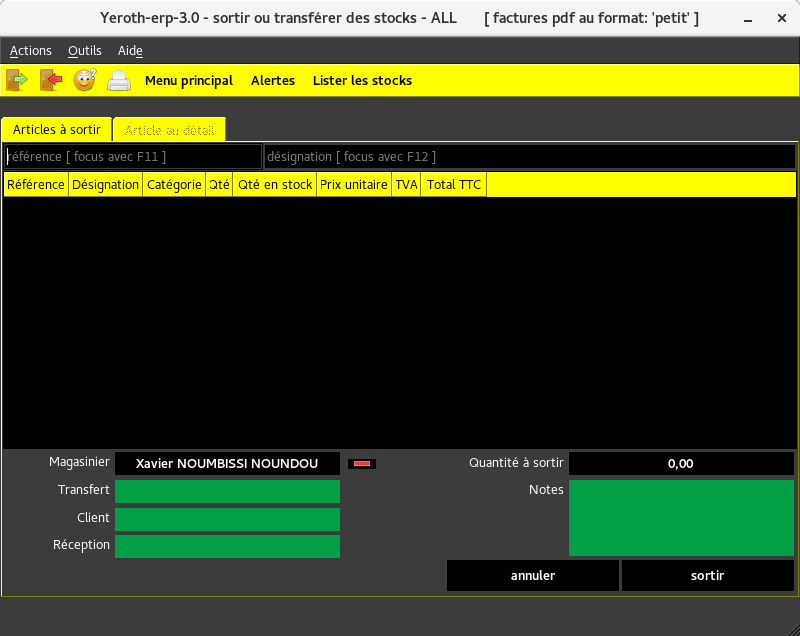
\includegraphics[scale=0.63]{images/yeren-fenetre-sortir-articles.png}
	\caption{La fen\^etre pour sortir des articles en stock.}
	\label{fig:yeren-fenetre-sortir-articles}
\end{figure}

La figure~\ref{fig:yeren-fenetre-sortir-articles} illustre
l'interface graphique pour proc\'eder aux sorties, ou aux
transferts d'articles.

La fen\^etre avec pour titre ''sortir ou transf\'erer des stocks''
permet d'effectuer les op\'erations suivantes:
\begin{enumerate}[1)]
	\item \textbf{une sortie de stocks};
	\item \textbf{un transfert de stocks}.\\
\end{enumerate}

Une \textbf{sortie de stocks} est le retrait d'articles
par un client aupr\`es d'une boutique (ou d'un d\'ep\^ot)
de votre entreprise apr\`es que le paiement se soit
effectu\'e dans une autre unit\'e de l'entreprise.

Un \textbf{transfert de stocks} est un mouvement de stocks
d'une boutique (ou d'un d\'ep\^ot) de votre entreprise
vers une autre unit\'e de l'entreprise.

\subsection{La strat\'egie de sortie des articles / stocks utilis\'ee}
\index{La strat\'egie de sortie des articles}
\index{La strat\'egie de sortie des stocks}

Le titre de la fen\^etre affiche la strat\'egie de sortie
des stocks utilis\'ee. La strat\'egie affich\'ee dans la
figure~\ref{fig:yeren-fenetre-sortir-articles} est: ''\cmup''
(en effet: \textbf{Cours Moyen Unit\'e Pond\'er\'e}).

%---------------------------------------------------

\nxsection{Effectuer une sortie d'articles}
\index{effectuer une sortie d'articles}
\index{effectuer une sortie de stock}

La d\'emarche pour effectuer une sortie d'articles en stock
est la suivante:
\begin{enumerate}[1)]
	\item s\'electionner les articles \`a faire sortir
	(appliquer l'une des m\'ethodes d\'ecrites dans
	la section~\ref{sec:selectionner-articles-vendre}
	du chapitre~\ref{chap:vendre} sur la vente d'article)

	\item le cas \'ech\'eant, choisissez le nom de
	l'entreprise cliente dans le menu d\'eroulant
	du champs de texte '\textbf{Client}'
	
	\item saisissez dans le champs de texte '\textbf{R\'ecepteur}'
	le nom de la personne qui r\'eceptionne les articles
	
	\item si vous avez des notes sp\'ecifiques \`a
	cette sortie d'articles, ecriver les dans 
	le champs de texte '\textbf{notes}'
	
	\item cliquer sur le bouton \bouton{Sortir}
	pour conclure la sortie de stocks.
\end{enumerate}

%---------------------------------------------------

\nxsection{Effectuer un transfert d'articles}
\index{effectuer un transfert d'articles}
\index{effectuer un transfert de stock}

La d\'emarche pour effectuer un transfert d'articles en stock
est la suivante:
\begin{enumerate}[1)]
	\item s\'electionner les articles \`a transf\'erer
	(appliquer l'une des m\'ethodes d\'ecrites dans la
	section~\ref{sec:selectionner-articles-vendre}
	du chapitre~\ref{chap:vendre} sur la vente d'article)
		
	\item saisissez dans le champs de texte
	'\textbf{R\'ecepteur}' le nom de la personne
	qui r\'eceptionne les articles
	
	\item sasissez ensuite dans le champs de texte
	'\textbf{Transfert}' le nom de la boutique ou
	du d\'ep\^ot qui recevra les articles \`a transferer
	
	\item si vous avez des notes sp\'ecifiques \`a
	ce transfert d'articles, ecriver les dans 
	le champs de texte '\textbf{notes}'
	
	\item cliquez sur bouton \bouton{Sortir}
	pour conclure le transfert d'articles.
\end{enumerate}

%---------------------------------------------------

\nxsection{Autres op\'erations de sortie d'articles / de stocks}
\index{autres op\'erations de sortie d'articles}
\index{autres op\'erations de sortie de stocks}

Pour toutes autres op\'erations de sortie des stocks,
appliquer la m\'ethode similaire d\'ecrite dans le
chapitre~\ref{chap:vendre} qui porte sur la vente d'articles
(ex.: annuler la sortie d'articles, imprimer une proforma
du bon de sortie, etc.).
